\subsection{Five-minute evaluation experiments: additional metrics}
These two earlier blocks each used a five-minute evaluation, one-minute warm-up and two-minute drain, with 210,000 admitted evaluation messages per trial. Each block contains its own unchanged-assignment baseline and its intervention, each run twice. They remain separate comparisons rather than being pooled into the later ten-minute experiments. Their diagnostics, process resources and retrospective completion-deadline sensitivity are included here for completeness.

The historical monitoring gaps are retained. Some predate the correction that initializes a returned-record position from a verified assignment offset while the client position remains unresolved. The correction was not applied retrospectively to invent missing values. Missing observations also restart the fifteen-observation persistence history, so the diagnostic gap may last longer than the ownership transfer itself. A shorter growth window cannot recover measurements that were never available. No comparison of these blocks with the later ten-minute blocks isolates duration alone: dates, selected partition identities and the monitoring implementation also changed.
\subsubsection{Five-minute evaluation: targeted scaling}
\begin{table}[!htbp]
\centering\small
\setlength{\tabcolsep}{3pt}
\renewcommand{\arraystretch}{1.12}
\begin{tabular}{@{}lrrrrr@{}}
\toprule
Response & Run & \shortstack{p99\\(s)} & \shortstack{Unfinished\\(\%)} & \shortstack{Misses $>1$ s\\(\%)} & \shortstack{Useful throughput\\(msg/s)}\\
\midrule
Keep 3 & 1 & 231.58 & 31.760 & 83.42 & 415.93\\
Targeted scale 6 & 1 & 110.70 & 0.000 & 57.01 & 757.32\\
Keep 3 & 2 & 229.28 & 31.037 & 83.24 & 418.90\\
Targeted scale 6 & 2 & 109.47 & 0.000 & 58.17 & 755.63\\
\bottomrule
\end{tabular}
\caption{Whole evaluation-born cohort through the fixed drain cutoff. Deadline misses include overdue unfinished messages. Useful throughput counts distinct completions during evaluation, including warm-up records completed then; it can exceed the input rate while queued work is cleared.}
\label{tab:short-targeted-scaling-outcomes}
\end{table}
\begin{table}[!htbp]
\centering\small
\setlength{\tabcolsep}{3pt}
\renewcommand{\arraystretch}{1.12}
\begin{tabular}{@{}lrrrrr@{}}
\toprule
Response & Run & \shortstack{Actual CPU\\(core-s)} & \shortstack{Actual RSS\\(GiB-min)} & \shortstack{Requested CPU\\(core-min)} & \shortstack{Requested memory\\(GiB-min)}\\
\midrule
Keep 3 & 1 & 515.3 & 1.57 & 42.00 & 21.00\\
Targeted scale 6 & 1 & 704.8 & 2.27 & 76.70 & 38.35\\
Keep 3 & 2 & 519.5 & 1.56 & --- & ---\\
Targeted scale 6 & 2 & 687.6 & 2.25 & 76.81 & 38.40\\
\bottomrule
\end{tabular}
\caption{Consumer resources over evaluation plus drain. Actual values integrate observed process CPU and RSS intervals and sum them across consumers. Requested values integrate Kubernetes resource declarations; neither is monetary or whole-cluster cost. A dash denotes unavailable full-window request coverage, not zero cost.}
\label{tab:short-targeted-scaling-resources}
\end{table}
\begin{table}[!htbp]
\centering\small
\setlength{\tabcolsep}{3pt}
\renewcommand{\arraystretch}{1.12}
\begin{tabular}{@{}lrrrrrr@{}}
\toprule
Response & Run & \shortstack{Mean total\\lag} & \shortstack{Peak total\\lag} & \shortstack{Lag coverage\\(\%)} & \shortstack{Peak partition\\lag} & Mean skew\\
\midrule
Keep 3 & 1 & 58,517 & 101,938 & 99.3 & 8,290 & 4.92\\
Targeted scale 6 & 1 & 19,438 & 50,671 & 86.0 & 4,960 & 8.47\\
Keep 3 & 2 & 57,077 & 99,351 & 99.3 & 8,047 & 4.93\\
Targeted scale 6 & 2 & 19,473 & 51,721 & 83.3 & 4,245 & 8.92\\
\bottomrule
\end{tabular}
\caption{Lag diagnostics during evaluation only, in offsets except skew and coverage. Means use trapezoidal area divided by covered time; peaks are sampled maxima. The time mean of the skew ratio is not the ratio of time-averaged maximum and mean lag. Invalid samples and ownership changes are not bridged.}
\label{tab:short-targeted-scaling-diagnostics}
\end{table}
\begin{figure}[p]
\centering
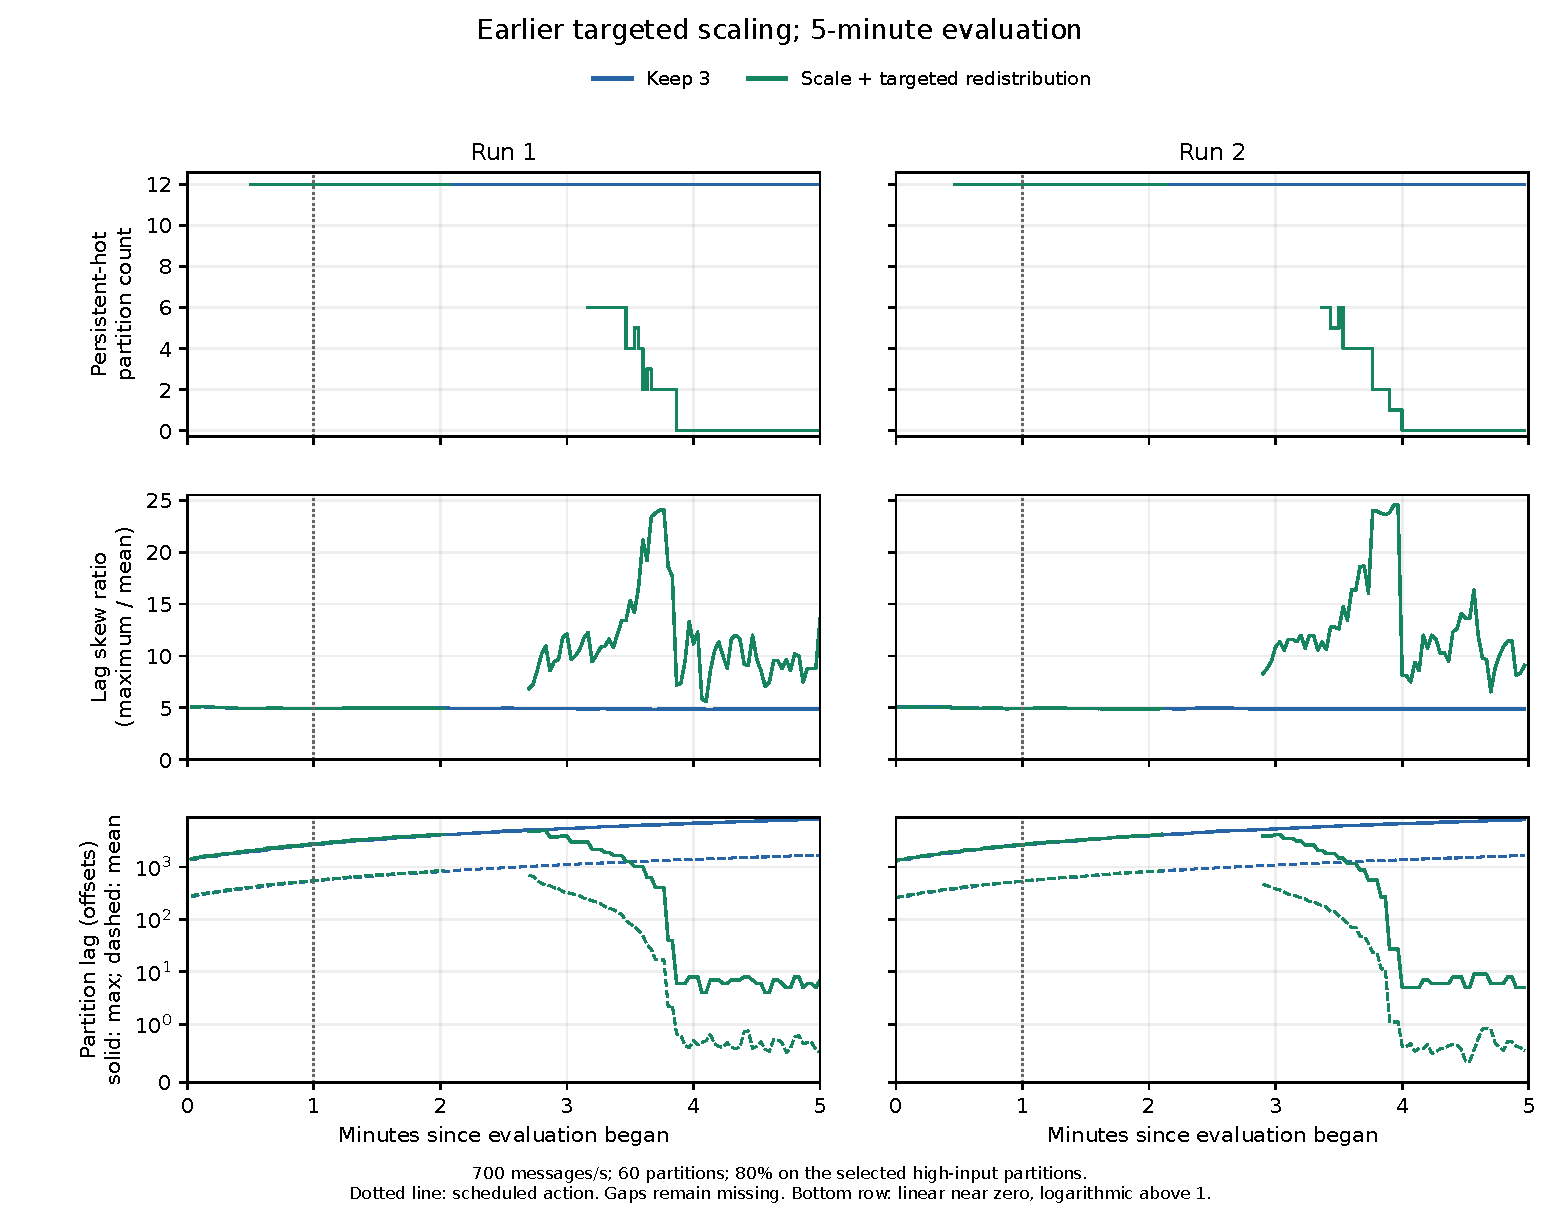
\includegraphics[width=\linewidth,height=.79\textheight,keepaspectratio]{figures/short-targeted-scaling-diagnostics.pdf}
\caption{Earlier five-minute evaluation with the original monitoring gaps retained. Persistent-hot counts, skew and maximum/mean partition lag are interpreted together.}
\label{fig:short-targeted-scaling-diagnostics}
\end{figure}
\clearpage
\subsubsection{Five-minute evaluation: redistribution}
\begin{table}[!htbp]
\centering\small
\setlength{\tabcolsep}{3pt}
\renewcommand{\arraystretch}{1.12}
\begin{tabular}{@{}lrrrrr@{}}
\toprule
Response & Run & \shortstack{p99\\(s)} & \shortstack{Unfinished\\(\%)} & \shortstack{Misses $>1$ s\\(\%)} & \shortstack{Useful throughput\\(msg/s)}\\
\midrule
Keep 3 & 1 & 226.34 & 30.182 & 83.41 & 422.08\\
Redistribute 3 & 1 & 103.76 & 0.000 & 61.59 & 725.25\\
Keep 3 & 2 & 227.13 & 30.475 & 83.24 & 421.76\\
Redistribute 3 & 2 & 91.38 & 0.000 & 60.84 & 727.54\\
\bottomrule
\end{tabular}
\caption{Whole evaluation-born cohort through the fixed drain cutoff. Deadline misses include overdue unfinished messages. Useful throughput counts distinct completions during evaluation, including warm-up records completed then; it can exceed the input rate while queued work is cleared.}
\label{tab:short-redistribution-outcomes}
\end{table}
\begin{table}[!htbp]
\centering\small
\setlength{\tabcolsep}{3pt}
\renewcommand{\arraystretch}{1.12}
\begin{tabular}{@{}lrrrrr@{}}
\toprule
Response & Run & \shortstack{Actual CPU\\(core-s)} & \shortstack{Actual RSS\\(GiB-min)} & \shortstack{Requested CPU\\(core-min)} & \shortstack{Requested memory\\(GiB-min)}\\
\midrule
Keep 3 & 1 & 515.8 & 1.56 & 42.00 & 21.00\\
Redistribute 3 & 1 & 554.1 & 1.47 & 42.00 & 21.00\\
Keep 3 & 2 & 516.5 & 1.55 & 42.00 & 21.00\\
Redistribute 3 & 2 & 553.4 & 1.46 & 42.00 & 21.00\\
\bottomrule
\end{tabular}
\caption{Consumer resources over evaluation plus drain. Actual values integrate observed process CPU and RSS intervals and sum them across consumers. Requested values integrate Kubernetes resource declarations; neither is monetary or whole-cluster cost. A dash denotes unavailable full-window request coverage, not zero cost.}
\label{tab:short-redistribution-resources}
\end{table}
\begin{table}[!htbp]
\centering\small
\setlength{\tabcolsep}{3pt}
\renewcommand{\arraystretch}{1.12}
\begin{tabular}{@{}lrrrrrr@{}}
\toprule
Response & Run & \shortstack{Mean total\\lag} & \shortstack{Peak total\\lag} & \shortstack{Lag coverage\\(\%)} & \shortstack{Peak partition\\lag} & Mean skew\\
\midrule
Keep 3 & 1 & 58,189 & 99,805 & 99.3 & 8,109 & 4.93\\
Redistribute 3 & 1 & 19,243 & 37,159 & 67.3 & 3,724 & 9.41\\
Keep 3 & 2 & 57,329 & 99,153 & 99.3 & 8,025 & 4.92\\
Redistribute 3 & 2 & 17,609 & 35,615 & 68.7 & 3,581 & 9.57\\
\bottomrule
\end{tabular}
\caption{Lag diagnostics during evaluation only, in offsets except skew and coverage. Means use trapezoidal area divided by covered time; peaks are sampled maxima. The time mean of the skew ratio is not the ratio of time-averaged maximum and mean lag. Invalid samples and ownership changes are not bridged.}
\label{tab:short-redistribution-diagnostics}
\end{table}
\begin{figure}[p]
\centering
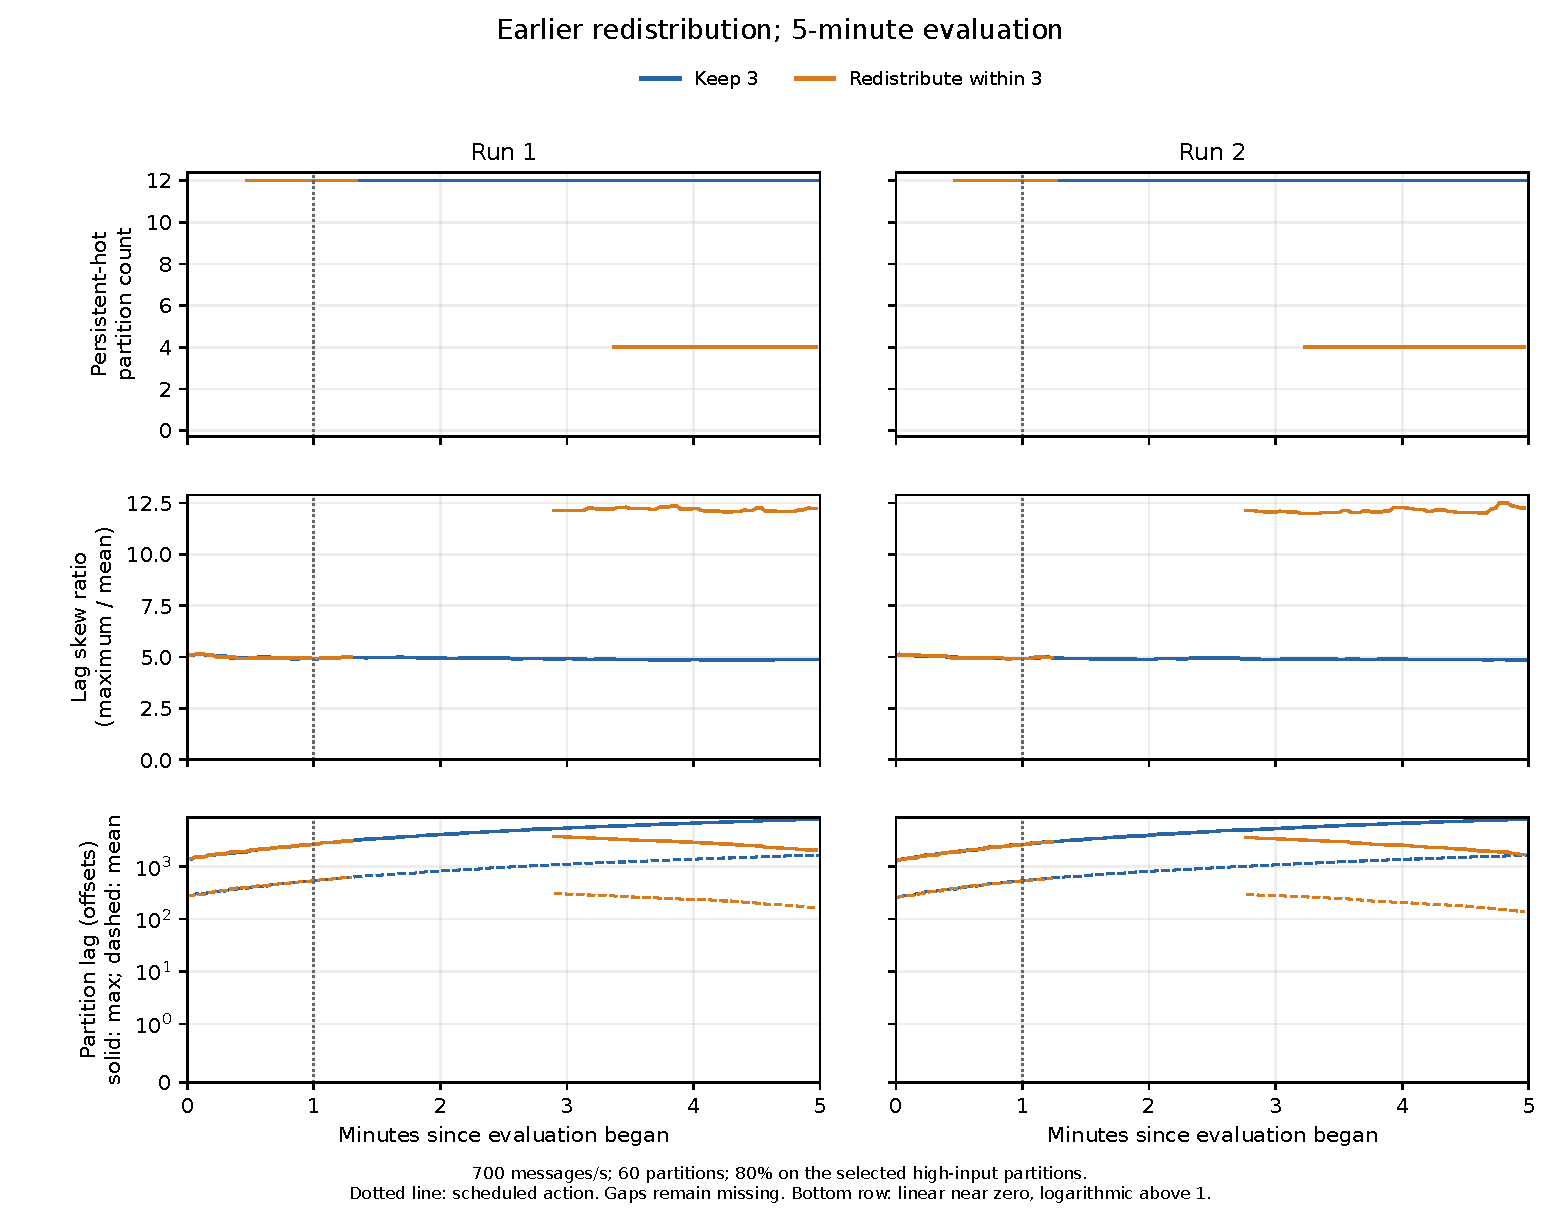
\includegraphics[width=\linewidth,height=.79\textheight,keepaspectratio]{figures/short-redistribution-diagnostics.pdf}
\caption{Earlier five-minute evaluation with the original monitoring gaps retained. Persistent-hot counts, skew and maximum/mean partition lag are interpreted together.}
\label{fig:short-redistribution-diagnostics}
\end{figure}
\clearpage
